\chapter*{Zpětná stereoprojekce}

Máme-li k dispozici několik obrazů téže scény, které byly získány několika kamerami umístěnými ve scéně nebo jedinou kamerou umístěnou postupně do různých míst, pak lze za jistých okolností provést rekonstrukci scény. Nejmenší počet kamer (případně míst), které jsou k provedení rekonstrukce zapotřebí, jsou dvě (obr. \ref{img:11_1}). Rekonstrukcí při tom rozumíme, že pro zvolené body dokážeme na základě souřadnic jejich obrazů zachycených kamerami vypočítat trojrozměrné souřadnice ve scéně. Řešení naznačeného problému podrobněji popíšeme v následujících podkapitolách.

\section*{Model kamery}

Předpokládáme, že vztah mezi objekty pozorovanými kamerou a jejich obrazy je lineární projektivní transformací (kolineací). Modelem kamery je tedy dírková komora. Ve scéně zavedeme globální souřadný systém (\textit{O},\textit{x},\textit{y},\textit{z}) (obr. \ref{img:11_1}). Uvažujme \textit{i}-tou kameru (případně \textit{i}-tou polohu kamery). Pro označení veličin vztahujících se k \textit{i}-té kameře použijeme symbolů s indexem \textit{i}. Střed projekce \textit{i}-té kamery je \textit{O}$_i$, $\pi_i$ je zobrazovací rovina. Kolmice vedená z \textit{O}$_i$ na rovinu $\pi_i$ je optická osa kamery. V zobrazovací rovině kamery leží zařízení zachycující obraz (jedná se například o pole snímacích elementů CCD čipu, případně o světlocitlivou vrstvu). Souřadnice bodů v obrazech měříme v souřadném systému (\textit{Z}$_i$,\textit{u}$_i$,\textit{v}$_i$). V případě CCD kamery  jsou často souřadné osy tohoto systému hranami pole snímacích elementů. Ortogonální souřadný systém (\textit{O}$_i$,\textit{x}$_i$,\textit{y}$_i$,\textit{z}$_i$) je souřadným systémem kamery. Jeho osa \textit{z}$_i$ je identická s optickou osou kamery, osa \textit{x}$_i$ je rovnoběžná s osou \textit{u}$_i$ (v případě CCD kamery tedy s hranou pole snímacích elementů). Dále v obraze zavedeme souřadný systém (\textit{O'}$_i$,\textit{x'}$_i$,\textit{y'}$_i$). Bod \textit{O'}$_i$ leží v místě, kde optická osa kamery protíná zobrazovací rovinu. Osa \textit{x'}$_i$ je rovnoběžná s osou  \textit{x}$_i$, osa \textit{y'}$_i$ je rovnoběžná s osou \textit{y}$_i$. Vzdálenost \textit{f}$_i$ = dist(\textit{O}$_i$,\textit{O'}$_i$) je ohniskovou vzdáleností kamery.

\begin{figure}[th]
    \begin{center}
        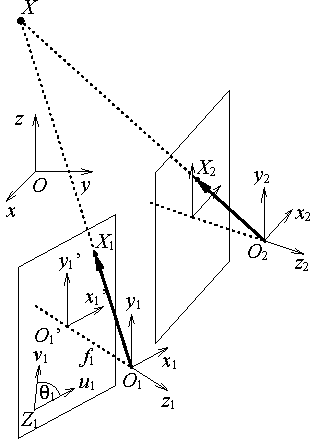
\includegraphics[scale=.9]{11_stereo/images/img_11_1.pdf}
    \end{center}
    \caption{Zpětná stereoprojekce.}
    \label{img:11_1}
\end{figure}

Uvažujme nějaký bod \textit{X} scény. V souřadném systému (\textit{O},\textit{x},\textit{y},\textit{z}) je bod \textit{X} reprezentován vektorem \textbf{x}=(\textit{x},\textit{y},\textit{z})$^\top$. V souřadném systému (\textit{O}$_i$,\textit{x}$_i$,\textit{y}$_i$,\textit{z}$_i$) je tentýž bod reprezentován vektorem \textbf{x}\textit{i}=(\textit{x}$_i$,\textit{y}$_i$,\textit{z}$_i$)$^\top$. Pro transformaci ze souřadného systému ($O_i$,$x_i$,$y_i$,$z_i$)  kamery do globálního souřadného systému (\textit{O},\textit{x},\textit{y},\textit{z}) scény můžeme psát

\begin{equation} \label{eq:11_1}
    \mathbf{x}=\mathbf{R}_{i} \mathbf{x}_{i} + \mathbf{o}_{i},
\end{equation}
kde matice \textbf{R}$_i$ popisuje rotaci kamery a vektor \textbf{o}$_i$ (zadaný v souřadném systému (\textit{O},\textit{x},\textit{y},\textit{z})) reprezentuje střed projekce $O_i$. Nechť \textit{X}$_i$ je bod v zobrazovací rovině \textit{i}-té kamery a tento bod nechť je obrazem bodu \textit{X} scény. Souřadnice bodu \textit{X}$_i$ měřené v souřadném systému ($Z_i$,$u_i$,$v_i$) jsou ($u_i$,$v_i$). Tyto souřadnice uspořádáme do trojrozměrného vektoru \textbf{u}\textit{i}=($u_i$,$v_i$,1)$^\top$. V souřadném systému ($O_i$',$x_i$',$y_i$') je poloha bodu \textit{X}$_i$ popsána vektorem $x_i' = (x_i', y_i', 1)^\top = \mathbf{Q}_i \mathbf{u}_i$, kde \textbf{Q}\textit{i} je matice popisující transformaci ze souřadného systému ($Z_i$,$u_i$,$v_i$) do souřadného systému ($O_i$',$x_i$',$y_i$'). Snadno ověříme, že platí

\begin{equation} \label{eq:11_2}
    Q_{i} = \left(
    \left[
    \begin{array}{ccc}
    {1} & {0} & {u_{0_{i} } } \\
    {0} & {1} & {v_{0_{i} } } \\
    {0} & {0} & {1}
    \end{array}
    \right]
    \left[
    \begin{array}{ccc}
    {1} & {0} & {0} \\
    {0} & {s_{i} } & {0} \\
    {0} & {0} & {1}
    \end{array}
    \right]
    \left[
    \begin{array}{ccc}
    {1} & {-\cot g\theta _{i} } & {0} \\
    {0} & {{1 \mathord{\left/{\vphantom{1 \sin \theta _{i} }}\right.\kern-\nulldelimiterspace} \sin \theta _{i} } } & {0} \\
    {0} & {0} & {1}
    \end{array}
    \right]
    \right)^{-1}
    =
    \left[
    \begin{array}{ccc}
    {1} & {-\cot g\theta _{i} } & {u_{0_{i} } } \\
    {0} & {{s \mathord{\left/{\vphantom{s \sin \theta _{i} }}\right.\kern-\nulldelimiterspace} \sin \theta _{i} } } & {v_{0_{i} } } \\
    {0} & {0} & {1}
    \end{array}
    \right]^{-1} .
\end{equation}

\begin{figure}[th]
    \begin{center}
        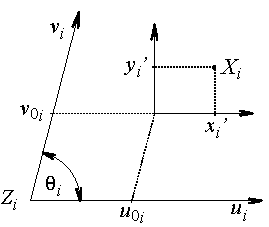
\includegraphics[scale=.9]{11_stereo/images/img_11_2.pdf}
    \end{center}
    \caption{K významu prvků matice $\mathbf{Q}_i$.}
    \label{img:11_2}
\end{figure}

Jednotlivé symboly v matici \textbf{Q}$_i$ mají následující význam (obr. \ref{img:11_2}). Hodnoty $u_{0i}$, $v_{0i}$ jsou souřadnice (měřené v souřadném systému ($Z_i$,$u_i$,$v_i$)) bodu, v němž optická osa protíná zobrazovací rovinu kamery. Úhel $\theta_i$ modeluje možnou odchylku pole snímacích elementů CCD senzoru od ortogonality, případně možnou úchylku kolmosti zobrazovací roviny a optické osy. Souřadný systém ($Z_i$,$u_i$,$v_i$) tedy nemusí být ortogonální, ale v praxi je hodnota $\theta_i$ obvykle velmi blízká $\pi$/2. Význam měřítkového faktoru \textit{s}$_i$ je následující: U kamer s CCD čipem zohledňuje možné diference rozměrů snímacích elementů ve směru osy \textit{u} a \textit{v}. Jestliže je výstup kamery analogový, pak parametr \textit{s}$_i$ zohledňuje také možné zkreslení rozměrů snímacích elementů způsobené následnou zpětnou digitalizací analogového signálu. Ze vztahu \eqref{eq:11_2} je zřejmé, že parametrem \textit{s}$_i$ korigujeme pouze poměrné zkreslení délek na osách - skutečná celková velikost obrazu bude vzata v úvahu hodnotou ohniskové vzdálenosti. Poznamenejme, že matice $Q_i^{-1}$ popisuje transformaci v opačném směru než matice $Q_i$, tedy ze souřadného systému (\textit{O}$_i$',$x_i$',$y_i$') do souřadného systému ($Z_i$,$u_i$,$v_i$). Zdá se názornější sestavit právě matici $Q_i^{-1}$. Matici \textbf{Q}$_i$ získáme inverzí. Tento postup jsme uplatnili ve vztahu \eqref{eq:11_2}. Zavedeme dále matici

\begin{equation} \label{eq:11_3}
    \mathbf{F}_{i} = \left[
    \begin{array}{ccc}
    {1} & {0} & {0} \\
    {0} & {1} & {0} \\
    {0} & {0} & {-f_{i}}
    \end{array}
    \right].  
\end{equation} 
Snadno ověříme, že platí

\begin{equation} \label{eq:11_4}
    \mathbf{x}_{i} =\lambda_{i} \mathbf{F}_{i} \mathbf{Q}_{i} \mathbf{u}_{i},
\end{equation}
kde $\lambda_{i}$ je reálný parametr. S využitím vztahu \eqref{eq:11_1} obdržíme

\begin{equation} \label{eq:11_5}
    \mathbf{x} = \lambda_{i} \mathbf{R}_{i} \mathbf{F}_{i} \mathbf{Q}_{i} \mathbf{u}_{i} + \mathbf{o}_{i},
\end{equation}
případně

\begin{equation} \label{eq:11_6}
    \lambda_{i} \mathbf{u}_{i} = \left(\mathbf{R}_{i} \mathbf{F}_{i} \mathbf{Q}_{i} \right)^{-1} \left(\mathbf{x} - \mathbf{o}_{i} \right).
\end{equation}

Parametry obsažené v maticích $\mathbf{F}_i$, $Q_{i}(f_i, u_{0i}, v_{0i}, \theta_i, s_i)$ jsou vnitřní (tzv. intrinsické) parametry kamery. Matice \textbf{Q}$_i$ zohledňuje některé rozdíly mezi skutečnou a ideální kamerou. V jednoduchých teoretických úvahách se někdy předpokládá \textbf{Q}$_i$=\textbf{I} (jednotková matice). Hodnoty \textbf{R}$_{i}$, \textbf{o}$_{i}$ popisující polohu kamer v prostoru se nazývají vnějšími (tzv. extrinsickými) parametry kamery. Základní úlohou počítačového stereovidění je na základě souřadnic ($u_i$,$v_i$) obrazů nějakého bodu scény zjistit jeho prostorové souřadnice (\textit{x},\textit{y},\textit{z}). K řešení této úlohy je zpravidla nejprve nutné provést tzv. kalibraci kamery. Úkolem kalibrace je stanovit vnitřní a vnější parametry kamery. Jen v případech, kdy jsou parametry kamery předem známy, může kalibrace chybět (od výrobce např. můžeme znát hodnoty vnitřních parametrů, umístění kamer v prostoru můžeme někdy dostatečně přesně změřit).

Vztahy popisující promítání realizované kamerou se zjednoduší, jestliže použijeme homogenních souřadnic. (Předpokládáme zde, že je čtenář obeznámen alespoň s elementárními pojmy  z projektivní geometrie. V případě potřeby lze potřebné znalosti získat např. z prací (Budínský 83, Penna 86)). Ostatně již dříve jsme vektor \textbf{u}$_{i}$ zavedli jako \textbf{u}$_{i}$=($u_i$,$v_i$,1)$^\top$, což lze interpretovat jako homogenní souřadnice bodu \textit{X}$_i$ v dvojrozměrném projektivním prostoru. Dále navíc připustíme, aby homogenní souřadnice nabývala obecné hodnoty \textit{w}$_i$, tedy $u_{i}=(w_i u_i, w_i v_i, w_i)^\top$. Podobně popíšeme v homogenních souřadnicích i polohu bodu \textit{X} vzhledem ke globálnímu souřadnému systému scény. Položíme \textbf{x}=(\textit{x},\textit{y},\textit{z},1)$^\top$. Projektivní transformaci realizovanou kamerou lze nyní zapsat ve tvaru

\begin{equation} \label{eq:11_7}
    \mathbf{u}_{i} = \mathbf{P}_{i} \mathbf{x}.
\end{equation}

Matice \textbf{P}$_{i}$ rozměru 3$\times$4 popisuje transformaci. Vztahy \eqref{eq:11_5}, \eqref{eq:11_6}, \eqref{eq:11_7} popisují různými prostředky tutéž transformaci a jsou vzájemně ekvivalentní.  V dalším textu budeme podle potřeby používat vždy ten tvar, který je pro danou úlohu nejvýhodnější. Porovnáním vztahu \eqref{eq:11_7} se vztahem \eqref{eq:11_6} zjišťujeme, že matice \textbf{P}$_{i}$ zahrnuje vliv vnějších i vnitřních parametrů kamery.

\section*{Případ dvou kamer s rovnoběžnými optickými osami} \label{sec:rovnobezne_kamery}

Nejprve ukážeme jednoduchý případ. Předpokládejme, že máme dvě kamery, které jsou uspořádány takto (obr. \ref{img:11_3}): 1) Obě kamery mají rovnoběžné optické osy. 2) Předpokládáme, že platí \textbf{Q}$_1$=\textbf{Q}$_2$=\textbf{I}, tedy \textit{x}$_1$'=\textit{u}$_1$, \textit{y}$_1$'=\textit{v}$_1$, \textit{x}$_2$'=\textit{u}$_2$, \textit{y}$_2$'=\textit{v}$_2$. 3) Souřadné osy \textit{u}$_1$, \textit{u}$_2$ leží v jedné přímce. 4) Souřadné osy \textit{v}$_1$,\textit{v}$_2$ jsou rovnoběžné. 5) Vzdálenost optických středů kamer je \textit{b}. 6) Počátek globálního souřadného systému scény půlí spojnici \textit{O}$_1$,\textit{O}$_2$ a osy globálního systému jsou rovnoběžné s osami \textit{u}$_1$(\textit{u}$_2$), \textit{v}$_1$(\textit{v}$_2$). 7)  \textit{f}$_1$=\textit{f}$_2$=\textit{f}. Uvažujme ve scéně bod \textit{X} o souřadnicích (\textit{x},\textit{y},\textit{z}). Bod \textit{X} se promítá do bodů \textit{X}$_1$, \textit{X}$_2$ ležících v~zobrazovacích rovinách první a druhé kamery. Souřadnice bodů \textit{X}$_1$, \textit{X}$_2$ měřené v obrazech získaných kamerami jsou (\textit{u}$_1$,\textit{v}$_1$), (\textit{u}$_2$,\textit{v}$_2$). Z podobnosti trojúhelníků snadno obdržíme následující vztahy (předpokládáme, že ohnisková vzdálenost \textit{f} se zadává jako kladná hodnota):

\begin{equation} \label{eq:11_8}
    \frac{x + b/2}{-z} = \frac{u_1}{f}, \quad \frac{x - b/2}{-z} = \frac{u_2}{f}.
\end{equation}

Analogické vztahy snadno zapíšeme také pro souřadnici \textit{y}. Máme

\begin{equation} \label{eq:11_9}
    \frac{y}{-z} = \frac{v_1}{f}, \quad \frac{y}{-z} = \frac{v_2}{f}.
\end{equation}

V rovnicích \eqref{eq:11_8} jsou \textit{x},\textit{z} neznámými. Ostatní hodnoty jsou známé. Řešením soustavy pro \textit{z} získáme

\begin{equation} \label{eq:11_10}
    z = - \frac{bf}{u_1 - u_2}.
\end{equation}

S využitím rovnic \eqref{eq:11_8}, \eqref{eq:11_9} pak snadno také nalezneme hodnoty \textit{x},\textit{y}. Vychází 

\begin{equation} \label{eq:11_11}
    x = \frac{b(u_1 + u_2)}{2(u_1 - u_2)}, \quad y = \frac{b(v_1 + v_2)}{2(u_1 - u2)}.
\end{equation}

\begin{figure}[th]
    \begin{center}
        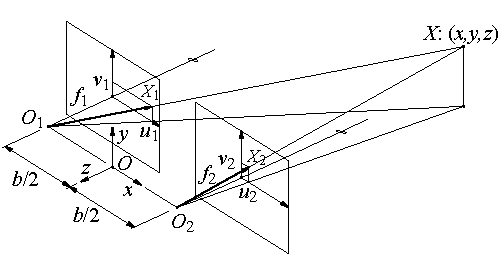
\includegraphics[scale=.9]{11_stereo/images/img_11_3.pdf}
    \end{center}
    \caption{Kamery s rovnoběžnými optickými osami.}
    \label{img:11_3}
\end{figure}

\section*{Absolutní kalibrace a rekonstrukce}

V tomto odstavci ukážeme postup, v němž se kalibrace provádí na základě toho, že pro jistý počet tzv. kalibračních bodů známe jak souřadnice $u_i$,$v_i$ jejich obrazů tak i jejich souřadnice \textit{x},\textit{y},\textit{z} v souřadném systému scény (název absolutní kalibrace je odvozen od požadavku znát souřadnice \textit{x},\textit{y},\textit{z} kalibračních bodů). Zaměříme se na případ, kdy máme pouze dvě kamery (\textit{i}=1,2). K odvození výsledných vztahů použijeme homogenních souřadnic a vyjdeme ze vztahu \eqref{eq:11_7}. Matici \textbf{P}$_{i}$ rozepíšeme do tří řádkových vektorů rozměru 1$\times$4 \textbf{P}$_{i}$=(\textbf{p}$_{i,1}$, \textbf{p}$_{i,2}$, \textbf{p}$_{i,3}$)$^\top$. Rovnici \eqref{eq:11_7} lze nyní přepsat takto

\begin{equation} \label{eq:11_12}
    \left[
    \begin{array}{c}
    {w_{i} u_{i} } \\
    {w_{i} v_{i} } \\
    {w_{i} }
    \end{array}
    \right]
    =
    \left[
    \begin{array}{c}
    {\mathbf{p}_{i,1} } \\
    {\mathbf{p}_{i,2} } \\
    {\mathbf{p}_{i,3} }
    \end{array}
    \right]
    \mathbf{x}.
\end{equation}

Předpokládejme nyní, že známe projekční matice \textbf{P}$_1$, \textbf{P}$_2$ obou kamer. Dále předpokládejme, že je ve scéně bod, jehož obraz získaný první kamerou má souřadnice \textit{u}$_1$,\textit{v}$_1$ a obraz získaný druhou kamerou má souřadnice \textit{u}$_2$,\textit{v}$_2$. Ukážeme, jak lze rekonstruovat trojrozměrné souřadnice \textit{x},\textit{y},\textit{z} tohoto bodu. Položme \textbf{x}=(\textit{x},\textit{y},\textit{z},1). Z posledního řádku rovnice \eqref{eq:11_12} máme

\begin{equation} \label{eq:11_13}
    w_{1} = \mathbf{p}_{1,3} \mathbf{x}, \quad w_{2} = \mathbf{p}_{2,3} \mathbf{x}.
\end{equation}
Dosazením rovnic \eqref{eq:11_13} do prvních dvou řádků vztahu \eqref{eq:11_12} rozepsaného pro první i druhou kameru dostaneme

\begin{equation} \label{eq:11_14}
    \left[
    \begin{array}{c}
    {\mathbf{p}_{1,1} \mathbf{x} - u_{1} \mathbf{p}_{1,3} \mathbf{x}} \\
    {\mathbf{p}_{1,2} \mathbf{x} - v_{1} \mathbf{p}_{1,3} \mathbf{x}} \\
    {\mathbf{p}_{2,1} \mathbf{x} - u_{2} \mathbf{p}_{2,3} \mathbf{x}} \\
    {\mathbf{p}_{2,2} \mathbf{x} - v_{2} \mathbf{p}_{2,3} \mathbf{x}}
    \end{array}
    \right]
    =
    \left[
    \begin{array}{c}
    {0} \\
    {0} \\
    {0} \\
    {0}
    \end{array}
    \right].  
\end{equation}

Vztah \eqref{eq:11_14} je lineární nehomogenní (uvažme, že \textbf{x}=(\textit{x},\textit{y},\textit{z},1)) soustavou rovnic pro neznámé hodnoty souřadnic \textit{x},\textit{y},\textit{z}. Protože pro tři neznámé jsou k dispozici čtyři rovnice, jde o soustavu předeterminovanou. Předeterminovanosti lze využít ke zmenšení vlivu chyb, které mohou být do výpočtu vneseny nepřesným zadáním. Hodnoty \textit{u}$_1$,\textit{v}$_1$, \textit{u}$_2$,\textit{v}$_2$ souřadnic měřených v obrazech bývají totiž zatíženy šumem, který vzniká nepřesným odečítáním souřadnic v obraze. Do této kategorie nepřesností patří i případ, kdy jsou v digitalizovaném obraze souřadnice měřeny pouze celočíselnými (nikoli reálnými) hodnotami (někdy udáváme souřadnice pixelu, do kterého obraz rekonstruovaného bodu padne, jako celočíselné). Řešení lineárních předeterminovaných systémů metodou nejmenších čtverců je popsáno v dodatku XXX B. XXX

Z předchozího výkladu vyplývá, že jsou-li k dispozici projekční matice \textbf{P}$_i$, pak lze provést rekonstrukci souřadnic bodů. Postup, v němž jsou projekční matice stanoveny, se obvykle nazývá kalibrací kamer. Ukážeme metodu, jak lze kalibraci provést. Dosaďme opět \eqref{eq:11_13} do prvních dvou řádků vztahu \eqref{eq:11_12} a proveďme transpozici obou takto získaných rovnic. Obdržíme

\begin{equation} \label{eq:11_15}
    \begin{array}{l}
    {\mathbf{x}^\top \mathbf{p}_{i,1}^\top - u_{i} \mathbf{x}^\top \mathbf{p}_{i,3}^\top =0,} \\
    {\mathbf{x}^\top \mathbf{p}_{i,2}^\top - v_{i} \mathbf{x}^\top \mathbf{p}_{i,3}^\top =0.}
    \end{array}
\end{equation}

Uspořádejme zatím neznámé prvky projekční matice \textbf{P}$_i$ do sloupcového vektoru \textbf{p}$_{i}$ = (\textbf{p}$^\top_{i,1}$, \textbf{p}$^\top_{i,2}$, \textbf{p}$^\top_{i,3}$)$^\top$. Vztahy \eqref{eq:11_15} lze pak přepsat maticově takto

\begin{equation} \label{eq:11_16}
    \left[
    \begin{array}{ccc}
    {\mathbf{x}^\top} & {\mathbf{0}^\top} & {-u_{i} \mathbf{x}^\top} \\
    {\mathbf{0}^\top} & {\mathbf{x}^\top} & {-v_{i} \mathbf{x}^\top}
    \end{array}
    \right]
    \left[
    \begin{array}{c}
    {\mathbf{p}_{i,1}^\top} \\
    {\mathbf{p}_{i,2}^\top} \\
    {\mathbf{p}_{i,3}^\top}
    \end{array}
    \right]
    =
    \left[
    \begin{array}{c}
    {0} \\
    {0}
    \end{array}
    \right].  
\end{equation} 

Rozepsáno tedy

\begin{equation} \label{eq:11_17}
    \left[
    \begin{array}{cccccccccccc}
    {x} & {y} & {z} & {1} & {0} & {0} & {0} & {0} & {-u_{i} x} & {-u_{i} y} & {-u_{i} z} & {-u_{i}} \\
    {0} & {0} & {0} & {0} & {x} & {y} & {z} & {1} & {-v_{i} x} & {-v_{i} y} & {-v_{i} z} & {-v_{i}}
    \end{array}
    \right]
    \mathbf{p}_{i}
    =
    \left[
    \begin{array}{c}
    {0} \\
    {0}
    \end{array}
    \right].
\end{equation} 

Vidíme, že každý kalibrační bod přispívá k nalezení prvků projekční matice dvěma rovnicemi. Stanovení dvanácti neznámých prvků projekční matice provedeme na základě rovnic poskytnutých dostatečným počtem kalibračních bodů. Ukážeme ale, že projekční matici bude možné pomocí kalibračních bodů stanovit až na reálného násobitele. Uvedenou nejednoznačnost lze snadno ilustrovat pomocí rovnice \eqref{eq:11_7}. Násobme levou i pravou stranu rovnice libovolným nenulovým reálným násobitelem $\mu$. Protože v homogenních souřadnicích vektor $\mu$\textbf{u}$_{i}$ reprezentuje tentýž bod obrazu jako vektor \textbf{u}$_{i}$, musí být také matice $\mu$\textbf{P}$_{i}$ nutně správnou projekční maticí. Nejednoznačnost vyřešíme zavedením doplňující podmínky. Snadno lze např. realizovat postup, kdy některý z prvků projekční matice položíme roven zvolené hodnotě (např. roven jedné). Jistou potíž však v tomto případě působí rozhodnutí, který ze členů projekční matice bychom měli takto nastavit (zejména se nesmíme pokoušet takto nastavit člen, který by měl vyjít nulový). Čistší možností je požadovat, aby vhodná norma projekční matice byla rovna zvolené hodnotě. Můžeme např. požadovat, aby součet čtverců všech prvků projekční matice byl roven jedné. V tomto případě však bohužel obdržíme nelineární úlohu, což je podstatná komplikace. Podkapitolu můžeme uzavřít konstatováním, že máme-li k dispozici pro každou kameru alespoň 6 kalibračních bodů a zvolíme-li doplňující podmínku, můžeme pro řešení prvků projekční matice sestavit systém rovnic a prvky jednoznačně vyřešit. I při použití minimálního počtu šesti bodů je ovšem tento systém předeterminovaný. Pro eliminaci šumu (šumem opět mohou být zatíženy zejména hodnoty souřadnic $u_i$,$v_i$ změřené v obrazech) bývá však v praxi počet kalibračních bodů mnohem vyšší než teoreticky nutné minimum. V otázce řešení předeterminovaných lineárních soustav opět odkazujeme na dodatek XXX B. XXX

\section*{Relativní kalibrace a rekonstrukce}

Často přichází v úvahu úloha, kdy můžeme měřit pouze souřadnice bodů v obrazech získaných kamerami. Trojrozměrné souřadnice žádného bodu ve scéně při tom nejsou k dispozici. Taková situace může nastat např. v případě vizuálního systému robota, který pracuje v neznámé scéně. Ukážeme, že i za této situace lze scénu rekonstruovat. Uvažujme opět situaci, kdy máme k dispozici dvě kamery, případně dva obrazy sejmuté ze dvou různých míst jedinou kamerou. Zavedeme matici rotace \textbf{R} a vektor posunutí \textbf{b} = \textit{O}$_2$ $-$ \textit{O}$_1$, které provádějí transformaci ze souřadného systému druhé kamery do souřadného systému první kamery podle vztahu

\begin{equation} \label{eq:11_18}
    \mathbf{x}_{1} = \mathbf{R} \mathbf{x}_{2} + \mathbf{b}.
\end{equation}

Připomeňme, že \textbf{R} je ortonormální matice a že \textbf{R} = \textbf{R}$_{z}$\textbf{R}$_{y}$\textbf{R}$_{x}$, kde \textbf{R}$_{x}$,\textbf{R}$_{y}$,\textbf{R}$_{z}$ jsou matice odpovídající postupně prováděným rotacím kolem os \textit{x}$_2$,\textit{y}$_2$ a \textit{z}$_2$. Zavedeme vektor $\varphi$ = ($\varphi_x$,$\varphi_{y}$,$\varphi_{z}$)$^\top$ obsahující odpovídající úhly rotace. Matice \textbf{R}$_{x}$, \textbf{R}$_{y}$, \textbf{R}$_{z}$ pak mají tvar

\begin{eqnarray} \label{eq:11_19}
    \mathbf{R}_{x}
    &=&
    \left[
    \begin{array}{ccc}
    {1} & {0} & {0} \\
    {0} & {\cos \varphi _{x} } & {\sin \varphi _{x}} \\
    {0} & {-\sin \varphi _{x} } & {\cos \varphi _{x}}
    \end{array}
    \right], \\
    \mathbf{R}_{y}
    &=&
    \left[
    \begin{array}{ccc}
    {\cos \varphi _{y} } & {0} & {-\sin \varphi _{y} } \\
    {0} & {1} & {0} \\
    {\sin \varphi _{y}} & {0} & {\cos \varphi _{y}}
    \end{array}
    \right], \\
    \mathbf{R}_{z}
    &=&
    \left[
    \begin{array}{ccc}
    {\cos \varphi _{z}} & {\sin \varphi _{z}} & {0} \\
    {-\sin \varphi _{z} } & {\cos \varphi _{z} } & {0} \\
    {0} & {0} & {1}
    \end{array}
    \right].
\end{eqnarray}

Jak ukážeme později, lze v procesu relativní kalibrace určit právě matici \textbf{R} a vektor \textbf{b}. Známe-li matici \textbf{R}$_1$ a vektor \textbf{o}$_1$ určující polohu první kamery v globálním souřadném systému scény, pak můžeme hodnoty \textbf{R}$_2$,\textbf{o}$_2$ ze vztahu \eqref{eq:11_1} určující polohu druhé kamery vyjádřit vztahy

\begin{equation} \label{eq:11_20}
    \mathbf{o}_{2} = \mathbf{R}_{1} \mathbf{b} + \mathbf{o}_{1} , \quad \mathbf{R}_{2} = \mathbf{R}_{1} \mathbf{R}.
\end{equation}

Hodnoty \textbf{R}$_1$,\textbf{o}$_1$ popisují vztah mezi souřadným systémem první kamery a globálním souřadným systémem scény. Tento vztah nelze v procesu relativní kalibrace určit. Někdy mohou být hodnoty \textbf{R}$_1$,\textbf{o}$_1$ známy předem. Jestliže tomu tak není, pak pro mnoho úloh postačí položit \textbf{R}$_1$ = \textbf{I} a \textbf{o}$_1$ = \textbf{0}, což znamená, že globální souřadný systém scény ztotožníme se souřadným systémem první kamery a souřadnice bodů ve scéně tak měříme v souřadném systému první kamery.

\begin{figure}[th]
    \begin{center}
        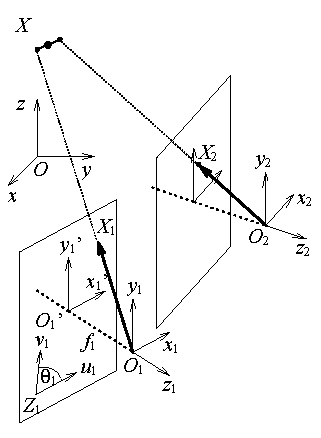
\includegraphics[scale=.9]{11_stereo/images/img_11_4.pdf}
    \end{center}
    \caption{Rekonstrukce polohy bodu.}
    \label{img:11_4}
\end{figure}

Předpokládejme nyní nejprve, že kalibrace již byla provedena a že matice \textbf{R}$_i$ a vektor \textbf{o}$_{i}$ (\textit{i}=1,2) z rovnice \eqref{eq:11_1} jsou již pro obě kamery známy. Nejprve ukážeme, jak lze provést rekonstrukci trojrozměrných souřadnic bodu, známe-li souřadnice jeho průmětů v obrazech získaných oběma kamerami. Nechť \textit{X} označuje rekonstruovaný bod. V souřadném systému (\textit{O},\textit{x},\textit{y},\textit{z}) nechť je bod \textit{X} reprezentován vektorem \textbf{x}=(\textit{x},\textit{y},\textit{z}). Nechť \textit{X}$_i$ je obraz bodu \textit{X} získaný \textit{i}-tou kamerou. V souřadném systému ($Z_i$,$u_i$,$v_i$) nechť je bod \textit{Xi} reprezentován vektorem \textbf{u}\textit{i}=($u_i$,$v_i$,1)$^\top$. V souřadném systému (\textit{O},\textit{x},\textit{y},\textit{z}) je přímka $\langle O_i X_i \rangle$ je popsána rovnicí \textbf{o}$_{i}$ + $\lambda_i \mathbf{R}_i \mathbf{F}_i \mathbf{Q}_i \mathbf{u}_i$, kde $\lambda_{i}$ je reálný parametr. Obě přímky $\langle O_i X_i \rangle$ (\textit{i}=1,2) by se teoreticky měly protínat v bodě \textit{X}. Opět je ovšem oprávněné předpokládat, že hodnoty souřadnic v obrazech nelze měřit zcela přesně. Proto nechť v tomto odstavci pojednávajícím o rekonstrukci souřadnic bodu značí \textbf{u}$_i$ prakticky zjištěné vektory souřadnic, jejichž složky jsou zatíženy šumem měření. Podobně bude nyní \textit{X}$_i$ značit prakticky zjištěnou polohu průmětu bodu \textit{X} v obraze získaném \textit{i}-tou kamerou. Je-li měření zatíženo chybami, pak již bod \textit{X} obecně nebude ležet současně na obou přímkách $\langle O_i X_i \rangle$ (obr. \ref{img:11_4}). Polohu bodu \textit{X} lze stanovit na základě podmínky, aby součet čtverců vzdáleností bodu \textit{X} od obou přímek byl minimální. Hledáme tedy minimum

\begin{equation} \label{eq:11_21}
    \min\limits_{\mathbf{x}} \sum_{i=1}^{2}\mathrm{dist}^{2} \left(\mathbf{x}, \mathbf{o}_{i} + \lambda_{i} \mathbf{R}_{i} \mathbf{F}_{i} \mathbf{Q}_{i} \mathbf{u}_{i} \right) .
\end{equation}

Pro stručnost matematických výrazů, které budou následovat, zavedeme vektor

\begin{equation} \label{eq:11_22}
    \mathbf{v}_{i} = \frac{\mathbf{R}_{i} \mathbf{F}_{i} \mathbf{Q}_{i} \mathbf{u}_{i}}{\left|\mathbf{R}_{i} \mathbf{F}_{i} \mathbf{Q}_{i} \mathbf{u}_{i} \right|} .  
\end{equation}

Na základě vlastností skalárního součinu pro hodnotu parametru $\lambda_{i}$ snadno nalezneme vztah

\begin{equation} \label{eq:11_23}
    \lambda_{i} = \left|\mathbf{x} - \mathbf{o}_{i} \right| \cos \varphi_{i} = \left(\mathbf{x} - \mathbf{o}_{i} \right)^\top v_{i} .
\end{equation}

\begin{figure}[th]
    \begin{center}
        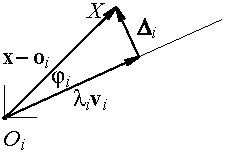
\includegraphics[scale=.9]{11_stereo/images/img_11_5.pdf}
    \end{center}
    \caption{Stanovení vzdálenosti bodu $X$ od promítacího paprsku.}
    \label{img:11_5}
\end{figure}

Nechť \textbf{$\Delta$}$_{i}$ označuje vektor vzdálenosti bodu \textit{X} od přímky $\langle O_i X_i\rangle$ (obr. \ref{img:11_5}). Je zřejmé, že \textbf{$\Delta$}$_{i}$ = (\textbf{x}$-$\textbf{o}$_{i}$) $-$ $\lambda_{i}$\textbf{v}$_{i}$. Součet čtverců vzdáleností můžeme nyní vyjádřit pomocí vztahů

\begin{eqnarray} \label{eq:11_24}
    \varepsilon &=& \sum_{i=1}^{2} \Delta_{i}^\top \Delta_{i} = \sum_{i=1}^{2} \left[ \left(\mathbf{x} - \mathbf{o}_{i} \right) - \lambda_{i} \mathbf{v}_{i} \right]^\top \left[ \left(\mathbf{x} - \mathbf{o}_{i} \right) - \lambda_{i} \mathbf{v}_{i} \right] = \nonumber \\ 
    &=& \sum_{i=1}^{2} \left[ \mathbf{x}^\top \mathbf{x} - 2 \mathbf{o}_{i}^\top \mathbf{x} - 2 \lambda_{i} \mathbf{v}_{i}^\top \mathbf{x} + \mathbf{o}_{i}^\top \mathbf{o}_{i} + 2 \lambda_{i} \mathbf{o}_{i}^\top \mathbf{v}_{i} + \lambda_{i}^{2} \mathbf{v}_{i}^\top \mathbf{v}_{i} \right] .
\end{eqnarray}

Derivováním získáme

\begin{equation} \label{eq:11_25}
    \frac{\partial \varepsilon}{\partial \mathbf{x}} = 2 \sum_{i=1}^{2} \left[ \mathbf{x} - \mathbf{o}_{i} - \frac{\partial \lambda_{i}}{\partial \mathbf{x}} \mathbf{v}_{i}^\top \mathbf{x} - \lambda_{i} \mathbf{v}_{i} + \frac{\partial \lambda_{i}}{\partial \mathbf{x}} \mathbf{o}_{i}^\top \mathbf{v}_{i} + \lambda_{i} \frac{\partial \lambda_{i}}{\partial \mathbf{x}} \mathbf{v}_{i}^\top \mathbf{v}_{i} \right] .
\end{equation}

Z rovnice \eqref{eq:11_23} vyplývá, že $\partial \lambda_{i}/\partial \mathbf{x} = \mathbf{v}_{i}$. Položíme-li $\partial \varepsilon/\partial \mathbf{x} = 0$, pak po úpravách obdržíme vztah

\begin{equation} \label{eq:11_26}
    \sum_{i=1}^{2} \left[ \mathbf{x} - \left( \mathbf{v}_{i}^\top \mathbf{x} \right) \mathbf{v}_{i} \right] = \sum_{i=1}^{2} \left[ \mathbf{o}_{i} - \left(\mathbf{o}_{i}^\top \mathbf{v}_{i} \right) \mathbf{v}_{i} \right] .
\end{equation}

Řešením rovnice \eqref{eq:11_26} získáme pro hledaný vektor \textbf{x} předpis

\begin{equation} \label{eq:11_27}
    \mathbf{x} = \left[ \sum_{i=1}^{2} \left( \mathbf{I} - \mathbf{v}_{i}^\top \mathbf{v}_{i} \right) \right]^{-1} \sum_{i=1}^{2} \left[ \mathbf{o}_{i} - \left( \mathbf{o}_{i}^\top \mathbf{v}_{i} \right) \mathbf{v}_{i} \right] .
\end{equation}

Nyní se vrátíme k problému kalibrace a ukážeme, jak lze zjistit matici \textbf{R} a vektor \textbf{b}, kterých lze podle rovnice \eqref{eq:11_20} použít ke zjištění matice \textbf{R}$_2$ a vektoru \textbf{o}$_2$ (jak jsme již dříve uvedli, předpokládáme, že matici \textbf{R}$_1$ a vektor \textbf{o}$_1$ známe). Uvažujme bod \textit{X} scény. V obrazech získaných první a druhou kamerou se tento bod zobrazuje na body \textit{X}$_1$,\textit{X}$_2$. V souřadném systému (\textit{O}$_1$,\textit{x}$_1$,\textit{y}$_1$,\textit{z}$_1$) jsou směry přímek $\langle O_1 X_1\rangle$, $\langle O_2 X_2\rangle$ reprezentovány vektory \textbf{x}$_1$, \textbf{Rx}$_2$. Jestliže jsou polohy bodů \textit{X}$_1$,\textit{X}$_2$ v obrazech určeny přesně, pak leží přímky $\langle O_1 X_1 \rangle$, $\langle O_2 X_2 \rangle$, $\langle O_1 O_2 \rangle$ v jedné rovině. Podmínku koplanarity lze matematicky zapsat vztahem \textbf{x}$_1.$(\textbf{b}$\times$(\textbf{Rx}$_2$)) = 0. Zápisem [\textbf{b}]$_\times$ označíme antisymetrickou matici realizující vektorový součin, tj. matici, která pro každý vektor \textbf{a} vyhovuje podmínce [\textbf{b}]$_\times$ \textbf{a} = \textbf{b} $\times$ \textbf{a}. Lze snadno ověřit, že platí

\begin{equation} \label{eq:11_28}
    \left[ \mathbf{b} \right]_{\times} = \left[
    \begin{array}{ccc}
    {0} & {-b_{z}} & {b_{y}} \\
    {b_{z}} & {0} & {-b_{x}} \\
    {-b_{y} } & {b_{x}} & {0}
    \end{array}
    \right].
\end{equation}

Přepíšeme-li nyní podmínku koplanarity do maticového tvaru, obdržíme rovnici \textbf{x}$_1^\top$[\textbf{b}]$\times$\textbf{Rx}$_2$ = 0. Dosadíme-li do podmínky rovnici \eqref{eq:11_4}, dostaneme

\begin{equation} \label{eq:11_29}
    \mathbf{u}_{1}^\top \mathbf{Q}_{1}^\top \mathbf{F}_{1}^\top \left[ \mathbf{b} \right]_{\times } \mathbf{RF}_{2} \mathbf{Q}_{2} \mathbf{u}_{2} =0,
\end{equation}

případně

\begin{equation} \label{eq:11_30}
    \mathbf{u}_{1}^\top \mathbf{Q}_{1}^\top \mathbf{F}_{1}^\top \left[ \mathbf{b} \right]_{\times} \mathbf{R}_{z} \mathbf{R}_{y} \mathbf{R}_{x} \mathbf{F}_{2} \mathbf{Q}_{2} \mathbf{u}_{2} = 0
\end{equation}

nebo také

\begin{equation} \label{eq:11_31}
    u_{1}^\top \mathbf{Cu}_{2} = 0, \quad \mathrm{kde} \quad \mathbf{C} = \mathbf{Q}_{1}^\top \mathbf{F}_{1}^\top \left[ \mathbf{b} \right]_{\times} \mathbf{RF}_{2} \mathbf{Q}_{2} = \mathbf{Q}_{1}^\top \mathbf{F}_{1}^\top \left[ \mathbf{b} \right]_{\times} \mathbf{R}_{z} \mathbf{R}_{y} \mathbf{R}_{x} \mathbf{F}_{2} \mathbf{Q}_{2}.
\end{equation}

Rovnice \eqref{eq:11_29}, \eqref{eq:11_30}, \eqref{eq:11_31} bývají nazývány rovnicemi koplanarity. Podobně bývá matice \textbf{C} z rovnice \eqref{eq:11_31} nazývána maticí koplanarity. Každá dvojice obrazů jednoho kalibračního bodu popsaná souřadnicemi \textbf{u}$_1$ v prvním obraze a souřadnicemi \textbf{u}$_2$ v druhém obraze dává vzniknout jedné rovnici koplanarity. Je-li k dispozici \textit{q} kalibračních bodů, pak lze sestavit soustavu \textit{q} rovnic koplanarity. Této soustavy lze pak použít k řešení neznámých vnějších a vnitřních parametrů kamery, které jsou obsaženy v maticích \textbf{Q}$_1$,\textbf{Q}$_2$,\textbf{F}$_1$,\textbf{F}$_2$,[\textbf{b}]$_\times$,\textbf{R}.

Z rovnice \eqref{eq:11_29} vyplývá, že řešení bude možné provést až na měřítko vektoru \textbf{b}. Jestliže je totiž \textbf{b} vektor, který vyhovuje rovnici \eqref{eq:11_29}, pak také vektor $\mu$\textbf{b}, kde $\mu$ je reálný násobitel, rovnici vyhovuje. Abychom úlohu specifikovali jednoznačně, zvolíme doplňující podmínku. Můžeme např. požadovat $\mid$\textbf{b}$\mid$=\textit{d}, kde \textit{d} je zvolená hodnota (např. \textit{d}=1). V případě euklidovské metriky lze pak podmínku rozepsat do tvaru

\begin{equation} \label{eq:11_32}
    b_{x}^{2} + b_{y}^{2} + b_{z}^{2} = d^{2} .
\end{equation}

Ze skutečnosti, že délku vektoru \textbf{b} je zapotřebí zvolit, vyplývá, že rekonstrukci scény bude možné provést až na měřítko. To znamená, že pro různé hodnoty \textit{d} budeme dostávat podobné, avšak různě veliké scény. Problém lze jednoduše vyřešit tak, že kalibraci provedeme při $\mid$\textbf{b}$\mid$=1. Známe-li pak skutečnou vzdálenost mezi některými dvěma body ve scéně, můžeme stanovit měřítko, kterým je třeba dodatečně násobit všechny souřadnice ve scéně (rozměry scény) tak, aby požadované vzdálenosti mezi body bylo skutečně dosaženo.

Z rovnice \eqref{eq:11_29} vidíme, že při relativní kalibraci lze stanovit vzájemnou polohu kamer a vnitřní parametry kamery. Vzájemná poloha kamer je popsána maticí \textbf{R} a vektorem \textbf{b}. Protože však může existovat nejvýše 7 nezávislých rovnic koplanarity (podrobný důkaz tohoto tvrzení neuvádíme, poněvadž by přesáhl rámec tohoto textu), lze pomocí rovnic koplanarity a s využitím doplňující podmínky \eqref{eq:11_32} zjistit nejvýše osm parametrů. To však nemusí být na závadu. Často lze totiž předpokládat, že se některé parametry (zejména vnitřní parametry kamery obsažené v maticích \textbf{Q}$_1$,\textbf{Q}$_2$) v čase nemění a lze je proto předem stanovit předchozím měřením (kalibrací) v laboratorních podmínkách.

Řešení soustavy kalibračních rovnic je obtížné, protože se jedná o nelineární problém. V posledním desetiletí bylo prezentováno několik přístupů k jeho řešení. Zde nastíníme jednu z možných variant. Vyjdeme z rovnic ve tvaru \eqref{eq:11_30}. Předpokládáme, že máme k dispozici \textit{q} kalibračních bodů. Souřadnice průmětů \textit{i}-tého kalibračního bodu v obraze první a druhé kamery označíme postupně \textbf{u}$_1^{(i)}$, \textbf{u}$_2^{(i)}$. Každá dvojice \textbf{u}$_1^{(i)}$, \textbf{u}$_2^{(i)}$ dává vzniknout jedné rovnici koplanarity. Dostaneme tak celkem \textit{q} rovnic koplanarity, kterých využijeme spolu s podmínkou \eqref{eq:11_32} ke stanovení hodnoty parametrů \textit{f}$_1$,\textit{f}$_2$,$\varphi_x$,$\varphi_y$,$\varphi_z$,\textit{b}$_x$,\textit{b}$_y$,\textit{b}$_z$. Je zřejmé, že nejmenší hodnota \textit{q}, při níž lze úlohu řešit, je 7. Prakticky však bývá \textit{q} vyšší. Předeterminovanosti soustavy lze opět využít k redukci vlivu šumu, kterým může být zatíženo měření souřadnic vektorů $u_1^{(i)}$, $u_2^{(i)}$. Hledané hodnoty parametrů uspořádáme do vektoru \textbf{p} = (\textit{f}$_1$,\textit{f}$_2$,$\varphi_x$,$\varphi_y$,$\varphi_z$,\textit{b}$_x$,\textit{b}$_y$,\textit{b}$_z$)$^\top$. Pro dvojici obrazů \textit{i}-tého kalibračního bodu můžeme pak rovnici \eqref{eq:11_30} zapsat přehledně ve tvaru

\begin{equation} \label{eq:11_33}
    F \left( \mathbf{u}_1^{(i)}, \mathbf{u}_2^{(i)}, \mathbf{p} \right) = 0.
\end{equation}

Podmínka \eqref{eq:11_32} spolu s \textit{q} (\textit{q}$>$7) rovnicemi \eqref{eq:11_33} tvoří předeterminovaný nekonzistentní systém (nekonzistence vyplývá z přítomnosti šumu ve vstupních hodnotách). Nekonzistentní systém nemá přísně vzato žádné řešení. Lze pouze najít řešení, které systému v jistém smyslu vyhovuje nejlépe. Můžeme například najít vektor parametrů \textbf{p} tak, aby součet čtverců reziduí rovnic \eqref{eq:11_33} byl minimální. Hledáme tedy takovou hodnotu vektoru parametrů, která minimalizuje funkci

\begin{equation} \label{eq:11_34}
    \Phi = \sum_{i=1}^{q} \left[ F\left( \mathbf{u}_1^{(i)}, \mathbf{u}_2^{(i)}, \mathbf{p} \right) \right]^2,
\end{equation}
a to za současného splnění podmínky \eqref{eq:11_32}. Hledání minima funkce za doplňujících podmínek lze provést metodou Lagrangeových multiplikátorů, která je popsána v dodatku C. Metoda převádí problém na problém nalezení prostého minima (bez doplňující podmínky) nové funkce, která však má větší počet argumentů. V našem případě je jistou komplikací, že je úloha nelineární. Nelineární úlohu minimalizace lze řešit např. gradientní metodou. Postup je popsán v dodatku XXX D. XXX

\section*{Epipolára}

Uvažujme bod \textit{X} scény. V obrazech získaných první a druhou kamerou jsou souřadnice průmětů tohoto bodu popsány vektory \textbf{u}1 = (\textit{u}$_1$,\textit{v}$_1$,1), \textbf{u}$_2$ = (\textit{u}$_2$,\textit{v}$_2$,1). Dosadíme-li do rovnice \eqref{eq:11_18} rovnici \eqref{eq:11_4} zapsanou pro první a druhou kameru, snadno získáme vztah

\begin{equation} \label{eq:11_35}
    \lambda_{1} \mathbf{F}_{1} \mathbf{Q}_{1} \mathbf{u}_{1} = \lambda_{2} \mathbf{RF}_{2} \mathbf{Q}_2 \mathbf{u}_{2} + \mathbf{b}.
\end{equation}
Odtud máme

\begin{equation} \label{eq:11_36}
    \lambda_2 \mathbf{u}_2 = \lambda_1 \mathbf{Q}_2^{-1} \mathbf{F}_2^{-1} \mathbf{R}^\top \mathbf{F}_1 \mathbf{Q}_{1} \mathbf{u}_1 - \mathbf{Q}_2^{-1} \mathbf{F}_2^{-1} \mathbf{R}^\top \mathbf{b}.
\end{equation}

Součin $\lambda_2 u_2$ ve vztahu \eqref{eq:11_36} reprezentuje v homogenních souřadnicích průmět bodu \textit{X} v obraze druhé kamery. Rovnice \eqref{eq:11_36} je homogenní parametrickou rovnicí přímky, v níž je parametrem hodnota $\lambda_1$. Můžeme tedy učinit tento závěr: Jestliže máme v obraze první kamery bod, jehož souřadnice jsou \textbf{u}$_1$ = (\textit{u}$_1$,\textit{v}$_1$,1), pak poloha jemu odpovídajícího bodu v obraze druhé kamery závisí na hodnotě $\lambda_1$ (použitím vztahu \eqref{eq:11_4} lze snadno ověřit, že platí $\lambda_1$ = $-$\textit{z}$_1$/\textit{f}$_1$). Všechny možné polohy vytvoří v obraze získaném druhou kamerou přímku. Tato přímka se nazývá epipolárou. Pro $\lambda_1$ = 0 rovnice \eqref{eq:11_36} určuje v obraze získaném druhou kamerou polohu průmětu středu projekce první kamery. Tento bod se nazývá epipól. Epipolára i epipól jsou vyobrazeny na obr. \ref{img:11_6}. Poznamenejme, že odvozené vztahy je samozřejmě možné také obrátit, což znamená, že k bodu v obraze získaném druhou kamerou je možné nalézt epipoláru v obraze získaném první kamerou. Totéž platí i pro epipól.

\begin{figure}[th]
    \begin{center}
        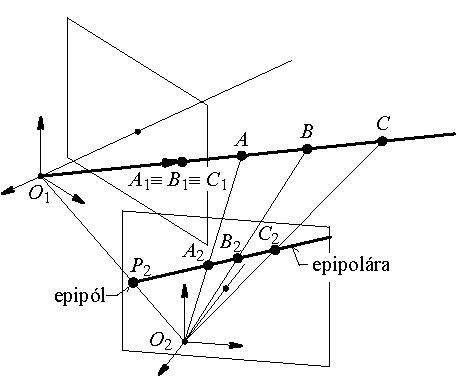
\includegraphics[scale=.9]{11_stereo/images/img_11_6.pdf}
    \end{center}
    \caption{Epipolára a epipól.}
    \label{img:11_6}
\end{figure}

V případě kamer s rovnoběžnými osami (podkapitola \ref{sec:rovnobezne_kamery}) se rovnice \eqref{eq:11_36} podstatně zjednoduší. V tomto případě totiž máme \textbf{F}$_1$ = \textbf{F}$_2$ (proto dále píšeme jen \textbf{F}), \textbf{Q}$_1$ =  \textbf{Q}$_2$ = \textbf{I} (jednotková matice) a \textbf{R} = \textbf{I}. Z rovnice \eqref{eq:11_36} obdržíme vztah $\lambda_2 \mathbf{u}_2 = \lambda_1 \mathbf{u}_1 - \mathbf{F}^{-1} \mathbf{b}$. Uvážíme-li, že \textbf{b} = (\textit{b}$_x$,0,0), pak z rovnice pro souřadnici \textit{z} zjišťujeme, že $\lambda_2 = \lambda_1$ (dále proto píšeme jen $\lambda$). Parametrické rovnice epipoláry pak jsou \textit{u}$_2$ = \textit{u}$_1$ $-$ \textit{b}$_x$ / $\lambda$, \textit{v}$_2$ = \textit{v}$_1$.

\section*{Automatizované hledání korespondence}

Pro rekonstrukci polohy bodu je zapotřebí identifikovat jeho průměty v obraze získaném první a druhou kamerou. Zdá se, že je možné uvažovat i o automatizaci této úlohy. Lze postupovat např. v následujících krocích: 1) V obraze získaném první kamerou identifikujeme body zájmu např. některým z detektorů rohů (kapitola 8.4). 2) Pro každý bod zájmu nalezený v prvním obraze určíme korespondující bod v druhém obraze. Druhý krok popíšeme podrobněji. Nechť \textit{X}$_1$ je bod zájmu nalezený v prvním obraze a jeho souřadnice nechť jsou \textit{u}$_1$,\textit{v}$_1$. Z předchozí podkapitoly víme, že korespondující bod \textit{X}$_2$ bude v druhém obraze ležet na epipoláře. Předpokládáme, že kromě hodnoty $\lambda_1$, která je parametrem, jsou všechny zbývající hodnoty na pravé straně rovnice \eqref{eq:11_36} k~dispozici (řekněme, že již byla provedena kalibrace). Můžeme proto stanovit rovnici epipoláry, na níž bod \textit{X}$_2$ leží. Přesnou polohu bodu \textit{X}$_2$ nalezneme tak, že systematicky prověřujeme všechny body na epipoláře (při praktické implementaci můžeme postupovat např. po celých pixelech). Označme $\varphi_1$(\textit{u},\textit{v}), $\varphi_2$(\textit{u},\textit{v}) obrazové funkce prvního a druhého obrazu. Nechť \textit{u},\textit{v} jsou souřadnice prověřovaného bodu ve druhém obraze. Otázku, zda prověřovaný bod koresponduje s \textit{X}1, můžeme rozhodnout na základě porovnání okolí bodu \textit{X}$_1$ s okolím bodu prověřovaného. K porovnání lze použít např. vztahu (obr. \ref{img:11_7})

\begin{equation} \label{eq:11_37}
    \mathrm{Diff} \left( u,v \right) = \sum_{\Delta u=-a}^{a} \sum_{\Delta v=-a}^{a} \left[ \varphi_1 \left( u_1 + \Delta u,v_1 + \Delta v \right) - \varphi_2 \left( u + \Delta u, v + \Delta v \right) \right]^2.
\end{equation}

Je zřejmé, že vztah \eqref{eq:11_37} porovnává okolí čtvercového tvaru o straně $2 a + 1$. Čím menší hodnota vyjde, tím jsou si okolí podobnější. Za bod korespondující s \textit{X}$_1$ lze považovat takový bod \textit{X}$_2$, který splňuje následující kriteria: 1) hodnota vypočítaná podle vztahu \eqref{eq:11_37} je pro \textit{X}$_2$ minimální a menší než nějaký zvolený práh, 2) pro všechny ostatní body na epipoláře je hodnota \eqref{eq:11_37} významně větší než pro bod \textit{X}$_2$. Druhé kriterium zohledňuje požadavek jednoznačnosti detekce.

\begin{figure}[th]
    \begin{center}
        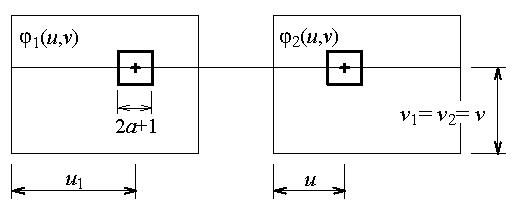
\includegraphics[scale=.9]{11_stereo/images/img_11_7.pdf}
    \end{center}
    \caption{Hledání korespondence porovnáním okolí bodu (kamery s rovnoběžnými optickými osami).}
    \label{img:11_7}
\end{figure}

Ačkoli právě popsaný postup vypadá dosti přímočaře, skrývá mnohá úskalí. Prvním problémem je volba vhodné velikosti okénka. Je-li okénko malé, hrozí, že detekce nebude jednoznačná. Při velkém okénku se naopak významněji uplatní fakt, že obrazy sejmuté z různých míst jsou přesně vzato různé a nelze obecně očekávat shodu příliš velkých oblastí ve smyslu vztahu \eqref{eq:11_37}. Vztah \eqref{eq:11_37} dále předpokládá, že okénku velikosti  2\textit{a}+1 v prvním obraze odpovídá ve druhém obraze okénko téže velikosti a že hrany okének jsou v obou obrazech rovnoběžné se souřadnými osami. To je splněno pouze ve speciálních případech (např. v případě kamer s rovnoběžnými optickými osami z podkapitoly \ref{sec:rovnobezne_kamery}).

\begin{figure}[th]
    \begin{center}
        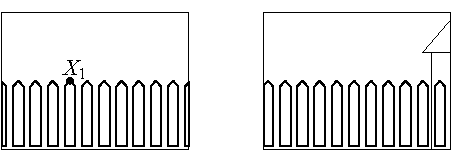
\includegraphics[scale=.9]{11_stereo/images/img_11_8.pdf}
    \end{center}
    \caption{K nejjednoznačnosti řešení problému korespondence.}
    \label{img:11_8}
\end{figure}

Otázka jednoznačnosti detekce korespondence je klíčová. Přísně vzato je zapotřebí se smířit s faktem, že mohou existovat případy, kdy jednoznačnou detekci zajistit nelze. Uvažme např. příklad dle obr. \ref{img:11_8}. Ani člověku se zde bez doplňujících informací nepodaří stanovit, který bod v~druhém obraze koresponduje s~bodem \textit{X}$_1$. Tím méně lze u podobných úloh očekávat řešení automatizované. Automatizované hledání korespondence je z výše uvedených důvodů úlohou, jejíž obecné řešení je obtížné. I když bylo pro automatizované hledání korespondence publikováno více postupů, nelze žádný z nich považovat za zcela uspokojivý.

\section*{Stereo korespondence BY MICHAL}

Na stereo korespondenci můžeme pohlížet jako na proces hledání podobnosti mezi dvěma skupinami dat v obrazech. Nalezení správné stereo korespondence je klíčovým článkem pro následnou 3D rekonstrukci scény. Zatímco náš mozek je schopen provádět tyto operace zcela automaticky, bez přispění vědomí, pro počítač je tento problém obtížně uchopitelný. Korespondenční algoritmy se ve zpracování obrazu vyvíjí více než 30 let a stále se nedá říct, že by se podařilo najít optimální řešení.

Stereo korespondenční metody se dělí podle typu výsledné disparitní mapy na husté (obsahující hodnotu disparity pro téměř všechny body v obraze) a řídké (disparita je přiřazena jen význačným bodům, hranám apod.). Další možností jak tyto algoritmy rozčlenit je na základě přístupu k hledání korespondence. Lokální metody hledají korespondenci jen na základě informací získaných z konečného okolí hledaného bodu, nejčastěji se jedná o malá čtvercová okénka. Globální metody přistupují k problému korespondence jako k optimalizačnímu problému, který má určit disparitu a zákryty na celé ploše obrazu. V následujících podkapitolách si ukážeme příklady obou přístupů.

\subsection*{Okénkové algoritmy}
Okénkové algoritmy vycházejí z předpokladu podobnosti okolí korespondujících bodů. Na prvním obraze vymezíme malou oblast, nejčastěji čtvercového tvaru, a tu postupně porovnáváme s potenciálními pozicemi, kde by se mohl nalézat korespondující bod druhého obrazu. Epipolární geometrie nám zajišťuje výskyt korespondujícího bodu na epipoláře, u rektifikovaných obrazů na stejné horizontální souřadnici. Pro porovnání oblastí okolí bodu se nejčastěji používají tři druhy metrik: rozdíl hodnot jasu (SAD, SSD), korelace (NCC) a metrika rank transformace. Máme-li definované okénko $u \times v$, jsme schopni určit míru podobnost pro danou hodnotu disparity $d$ pro jednotlivé metriky takto: 

\begin{equation}
    \label{e2}
	\mbox{\textit{SAD}}(u,v) =  \sum\limits_{u,v} \mid \varphi_{1}(u,v) - \varphi_{2}(u + d,v) \mid
\end{equation}

\begin{equation}
    \label{e1}
	\mbox{\textit{SSD}}(u,v) =  \sum\limits_{u,v} (\varphi_{1}(u,v) - \varphi_{2}(u + d,v))^2
\end{equation}

\begin{equation}
    \label{e3}
	\mbox{\textit{NCC}}(u,v) =  \sum\limits_{u,v} \frac{(\varphi_{1}(u,v) - \bar{\varphi_{1}}) \cdot (\varphi_{2}(u + d,v) - \bar{\varphi_{2}})}{\sqrt{(\varphi_{1}(u,v) - \bar{\varphi_{1}})^{2} \cdot (\varphi_{2}(u + d,v) - \bar{\varphi_{2}})^{2} } }
\end{equation}

Algoritmy využívající předchozí metriky jsou jednoduše implementovatelné a snadno paralelizovatelné. Nicméně, hlavní slabina těchto metod tkví ve volbě velikosti použitého okna. Malá okénka mají menší diskriminační schopnost a  budou vytvářet větší počet chybných korespondencí. Oproti tomu velká okénka mají sice větší odolnost proti šumu a poruchám v obraze, také ale rozmazávají disparitní mapu, protože nejsou schopny zachytit dostatečně jemně změnu disparity. Na obrázku \ref{img:stereo_demo_window} je výsledná disparitní mapa při použití metriky SAD. Z obrázku je patrné, že lokální metody selhávají na velkých jednolitých plochách. Problém volby velikosti porovnávaného okénka se snaží řešit algoritmy mající adaptivní velikost okna, jehož velikost a tvar se mění podle potřeby, nejčastěji na základě členitosti disparitní mapy a průběhu jasové funkce porovnávaných obrazů.

Kromě klasických metod využívající přímo jasové hodnoty pixelů, existují i alternativní metody, využívající neparametrické transformace vstupních obrazů. 
Příkladem je rank transformace. Rank transformace udává počet bodů v malém okénku kolem centrálního bodu, jejichž jasová hodnota je menší než jasová hodnota středového bodu. Výsledná hodnota tak závisí pouze na relativním uspořádání jasových hodnot, a ne na hodnotách samotných. Poté, co je provedena tato transformace, je možné bloky porovnávat běžnou $L_{1}$ normou.

\begin{eqnarray}
\mathrm{Rank}(u,v) &=&  \sum\limits_{u, v} (\varphi'_{1}(u,v) - \varphi'_{2}(u + d,v))^2, \\
\varphi'_{k}(u,v) &=& \sum\limits_{m, n} \mathrm{R}(m,n,u,v),\\
\mathrm{R}(m,n,u,v) &=& \left\{
\begin{array}{cc}
  0 & \varphi_{k}(m,n) \ge \varphi_{k}(u,v), \\
  1 & \varphi_{k}(m,n) < \varphi_{k}(u,v)
 \end{array}
 \right.
\end{eqnarray}

Výhodou rank transformace je větší odolnost proti šum. Z důvodu ztráty části informací je však snížena i rozlišovací schopnost porovnávání. 

\begin{figure}[bh]
    \centering
    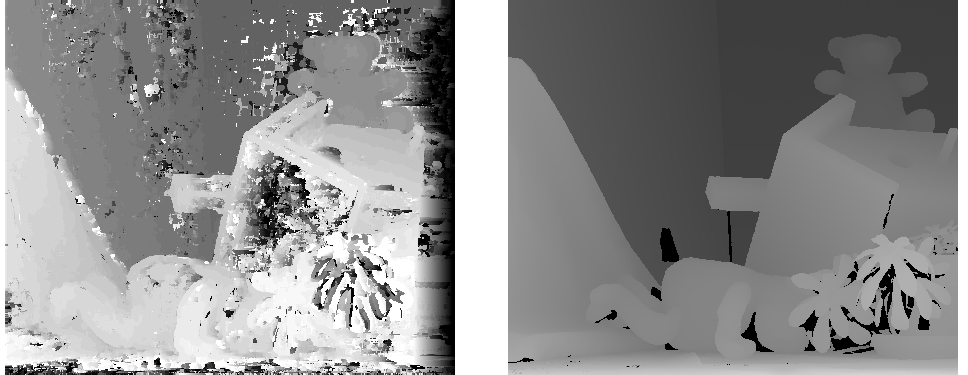
\includegraphics[width=5in]{11_stereo/images/stereo_demo_window}
    \caption{Výsledná disparitní mapa SAD a správné řešení.}
    \label{img:stereo_demo_window}
\end{figure}



\subsection*{Dynamické programování}
Dynamické programování je programovací technika, která se často užívá pro řešení optimalizačních úloh. Tuto techniku lze použít tehdy, lze-li původní úlohu rozložit na menší podúlohy, z jejichž optimálních řešení se poté složí řešení celé původní úlohy. Základem je Bellmanův princip optimality, který říká, že podstrategie optimální strategie je opět optimální. Využití dynamického programování vede k časově efektivnějším algoritmům, zpravidla však za cenu mírného zvýšení paměťových nároků. 

Předtím, než se podíváme na princip této metody, je třeba zavést některá omezení, bez kterých by tato metoda nebyla použitelná. Při hledání korespondence budeme předpokládat, že bod $X_{1}$ může korespondovat pouze s jedním bodem $X_{2}$ druhého obrazu. Zanedbáváme tím situace, ke kterým může docházet v případech, kdy se objekt snímaný jednou kamerou promítne do podoby jednoho pixelu, zatímco druhá kamera jej vlivem natočení vidí jako pixely dva. Dále musíme předpokládat, že změny v obrazech způsobené rozdílným umístěním kamer jsou natolik malé, že nedochází k záměně pořadí bodů ležících na epipoláře. Nachází-li se dva body $A$ a $B$ (oba leží na epipoláře) v těsné blízkosti, a bod A je situován vlevo od bodu B, předpokládáme, že na druhém snímku bude bod $A$ ležet opět vlevo od bodu $B$. Jako poslední omezení se často klade požadavek, aby výsledná disparitní mapa byla hladká, tj. disparita sousedních bodů se příliš neodlišovala.

\begin{figure}[htb]
    \centering
    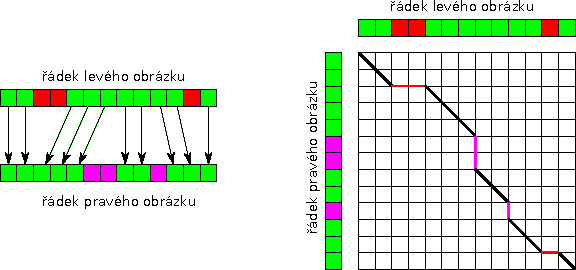
\includegraphics[width=4in]{11_stereo/images/stereo}
    \caption{Optimální cesta v síti.}
    \label{img:stereo}
\end{figure}

Za předpokladu splnění předchozích podmínek, jsme nyní schopni problém korespondence 
 převést na problém nalezení optimální cesty v síti. Hledání korespondence probíhá po jednotlivých řádcích. Podívejme se na příklad na obr. \ref{img:stereo}. Vidíme zde řádky levého a pravého obrazu a vyznačené korespondence mezi jednotlivými body. Barevně odlišeny jsou ty body, ke kterým nelze najít korespondující bod z důvodu zákrytu. Stejnou situaci ilustruje i síť zobrazená v pravé části obrázku.

Algoritmus, využívající dynamického programování, pak funguje následovně: Pro každý řádek levého ($I_{l}$) a pravého ($I_{r}$) obrazu vypočítáme matici $M_{h}$ velikosti $W \times W$, kde hodnota $W$ odpovídá šířce vstupních obrazů.
Matice $M_{h}$ je maticí cen korespondence mezi pixely $p(x,y)$ a $q(x + d,y)$ a hodnotou disparity $d$, přičemž $x + d < W$. Cena $M_{h}$ je definována jako  
\begin{equation}
    \label{cena}
    M_{h}(i,j) = \mbox{min}( \mbox{Diff}(i,j) + M_{h}(i-1, j-1), \lambda + M_{h}(i-1, j), \lambda + M_{h}(i, j-1)),
\end{equation}

kde $\lambda$ je hodnota penalizace, která se započítává pokud není nalezena korespondence a $\mbox{Diff}(i,j)$ je funkce porovnávající body, například pomocí podobnosti jejich okolí (SAD, SSD). Implementace výpočtu matice $M_{h}$ je ilustrována na výpisu \ref{alg1}.

\lstset{language=C,caption={DP -- Výpočet matice $M_{h}$},label=alg1}
\begin{lstlisting}
    for (int i = 1; i < W; i++)
        for (int j = 1; j < W; j++) {
            min1 = diff(i, j) + M[j-1, i-1 ];
            min2 = lambda + M[j-1, i ];
            min3 = lambda + M[j, i-1 ];
            M[i, j] = min(min1, min2, min3);
            D[i, j] = argmin(min1, min2, min3);
        }
\end{lstlisting}

Disparitní mapu pro daný řádek získáme zpětným průchodem matice $M_{h}$. Zpětný průchod začíná na pozici $M_{h}(W,W)$ a pokračuje po směru nejlevnější cesty. Pro implementaci je vhodné si zaznamenávat kromě ceny i směr, kterým jsme se do dané buňky dostali (v kódu matice $D$). Hodnotu disparity určíme během zpětného průchodu jako rozdíl souřadnic korespondujících bodů $d = i - j$. Výpis \ref{alg2} obsahuje možnou implementaci zpětného průchodu matice $M_{h}$ na základě směru určeného pomocí matice $D$.

\lstset{language=C,caption={DP -- Zpětný průchod},label=alg2}
\begin{lstlisting}
   i = j = W;
   while ( (i != 0) && (j != 0)) {
        switch (D[i, j]) {
            case 1:     
                    i--; j--; break;
            case 2:
                    i--; break;
            case 3:
                    j--; break;
            }
            d = i - j;
    }
\end{lstlisting}

Dynamické programování poskytuje lepší výsledky než běžné okénkové metody díky minimalizaci ceny korespondence. Zpracování každého řádku obrazu je nezávislé a lze takto snadno algoritmus paralelizovat. Jednou z nevýhod této metody je, že v základním provedení se provádí optimalizaci jen v rámci řádku a nebere se ohled na okolní výsledky. Ukázka výsledné disparitní mapy je na obr. \ref{img:stereo_demo_dp}.

\begin{figure}[htb]
    \centering
    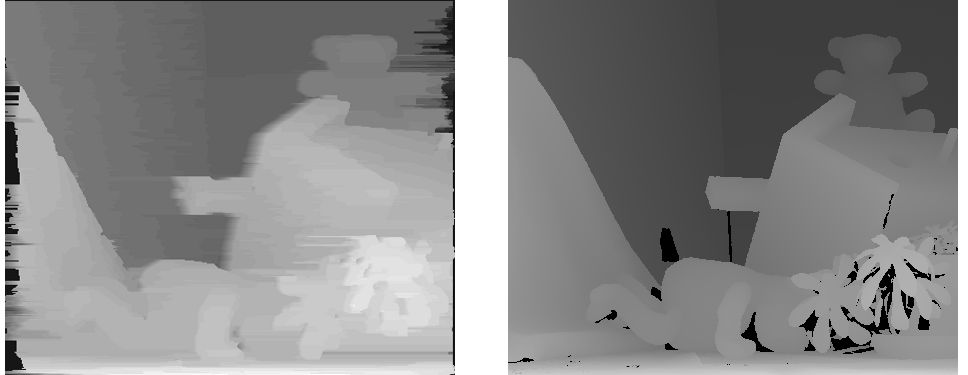
\includegraphics[width=5in]{11_stereo/images/stereo_demo_dp}
    \caption{Výsledná disparitní mapa DP a správné řešení.}
    \label{img:stereo_demo_dp}
\end{figure}

\subsection{Globální metody}
Globální metody hledají minimum funkce ceny ohodnocení disparity celého obrazu. V kontextu globálních metod se berou nejčastěji do úvahy tyto dvě podmínky: 
\begin{itemize}
	\item datová podmínka -- dva body korespondují tehdy, mají-li podobnou intenzitu všech složek; 
	\item požadavek hladkosti -- výsledná disparitní mapa by měla být po částech hladká, tedy dva sousední body musí mít pokud možno co jak nejvíce podobné hodnoty disparity.
\end{itemize}


Tyto dvě podmínky tvoří základ funkce, reprezentující celkovou energii přiřazení disparit. Algoritmy hledají takovou disparitní funkci $d$, která minimalizuje funkcionál $E(d)$ daný vztahem

\begin{equation}
    \label{funkcional}
	E(d) = E_\mathrm{d}(d) + \lambda E_\mathrm{s}(d),
\end{equation}

kde $E_\mathrm{d}(d)$ reprezentuje datovou podmínku, $E_\mathrm{s}(d)$ předpoklad hladkosti a konstanta $\lambda$ udává váhu hladkosti.

Hodnota $E_\mathrm{d}(d)$ udává podobnost dvou pixelů, kterou je možné vypočítat pomocí dříve zmíněných metrik (SSD, SAD apod.). Funkce $E_\mathrm{s}(d)$ pak může vypadat následovně:

\begin{equation}
    \label{funkcional2}
	E_\mathrm{s}(d) = \sum\limits_{u, v}  \rho(d(u,v) - d(u+1, v)) + \rho(d(u,v) - d(u, v+1)),
\end{equation}

kde $\rho$ je monotónně rostoucí funkce rozdílu disparit sousedních pixelů. Platí, že čím více se liší hodnota disparit sousedních pixelů, tím větší je i hodnota $E_\mathrm{s}(d)$.

Ukázalo se, že minimalizace funkcionálu $E(d)$ je NP-obtížný problém. Z tohoto důvodu se pro nalezení řešení užívají různé aproximační metody, jakými jsou grafové řezy, propagace zpráv, simulace žíhání a další. Není v možnostech těchto skript popsat tyto metody podrobněji a proto zde odkazujeme čtenáře na příslušnou literaturu.

